\part{Spazi Metrici}
\chapter{Spazi Metrici}

\section{Preliminari}
\definition
Si dice spazio metrico un insieme X non vuoto in cui sia definita una
distanza(metrica), vale a dire una funzione $d: X \times X \rightarrow \R$ con le proprietà:
\begin{enumerate}
	\item $d(x,y)\ge0 \quad \forall x,y \in X$
	\item $d(x,y)=0\Leftrightarrow x=0 \quad \forall x,y \in X$
	\item $d(x,y)=d(y,x) \quad \forall x,y \in X$ simmetria
	\item $d(x,y)\le d(x,z)+d(z,y) \quad \forall x,y,z\in X$ disuguaglianza triangolare 
\end{enumerate}

\example
$$X=\bbsetn{R}{2},\quad d((x_1,y_1),(X_2,y_2))=\sqrt{(x_2-x_1)^2+(y_2-y_1)^2}$$
si dimostra che la funzione così definita è una distanza:
\begin{enumerate}
	\item $d(x_1,x_2)\ge 0$, è verificata poiché l'argomento della radice è sempre positivo o al più nullo essendo una somma di quadrati, e la radice mantiene le quantità positive.
	\item $d((x_1,y_1),(x_2,y_2))=0\Leftrightarrow \sqrt{(x_2-x_1)^2+(y_2-y_1)^2}=0$\\
	$\Leftrightarrow (x_2-x_1)^2+(y_2-y_1)^2=0 $
	$\Leftrightarrow \left\{\begin{matrix}
	(x_2-x_1)^2=0\\
	(y_2-y_1)^2=0\\
	\end{matrix}\right.\Leftrightarrow
	\left\{\begin{matrix}
	x_2=x_1\\
	y_2=y_1\\
	\end{matrix}\right.$
	$\Leftrightarrow (x_1,y_1)=(x_2,y_2)$
	\item invertendo le prime componenti con le seconde, il quadrato non cambia quindi la simmetria è rispettata 
	$$d((x_1,y_1),(x_2,y_2))=\sqrt{(x_2-x_1)^2+(y_2-y_1)}=\sqrt{(x_1-x_2)^2+(y_1-y_2)}=d((x_2,y_2),(x_1,y_1))$$
	\item 
		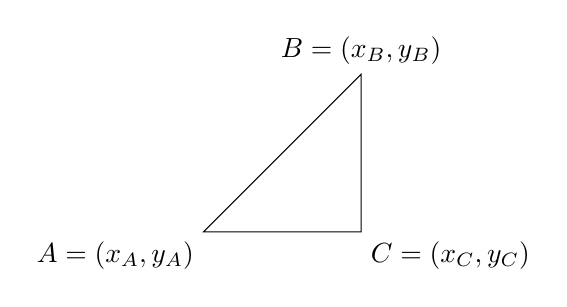
\begin{tikzpicture}[scale=0.5]
			\centering
		\draw (0,0) node[anchor=north east]{$A=(x_A,y_A)$}
			-- (4,0) node[anchor=north west]{$C=(x_C,y_C)$}
			-- (4,4) node[anchor=south]{$B=(x_B,y_B)$}
			-- cycle;
		\end{tikzpicture}
		... ci vorrebbe anche una spiegazione ... 
\end{enumerate}

\example
$$X=\R,\quad d(x_1,x_2)=\abs{x_2-x_1}$$
Le  proprietà 1,2,3 sono soddisfatte per le proprietà del modulo.\\
La proprietà 4 si può dimostrare: $$d(x_1,x_3)=\abs{x_3-x_1}\le\abs{x_3-x_2}+\abs{x_2-x_1}=d(x_3,x_2)+d(x_2,x_1)$$

\example
$$X=\bbsetn{R}{3}\quad d({x_1,y_1,z_1),(x_2,y_2,z_2)}$$
Analogo al primo esempio

\example
$$X=\bbsetn{R}{n}\quad$$
$$x=(x_1,\ldots,x_n) \quad\quad y=(y_1,\ldots,y_n)$$
$$d(x,y)=\sqrt{\sum\limits_{i=1}^{n}{\left(y_i-x_i\right)}^2}$$
Analogo al primo esempio

\example
$$X=\cntclass{0}(\realintervalclose{a}{b},\R),a,b\in\R, a<b$$
$$d_\infty=\sup\limits_{x\in\realintervalclose{a}{b}}\abs{g(x)-f(x)}$$
\begin{enumerate}
	\item $X$ contiene infiniti elementi(funzioni)
	\item $d_\infty$ è detta distanza uniforme o distanza della convergenza infinita o distanza della convergenza uniforme
	\item 
		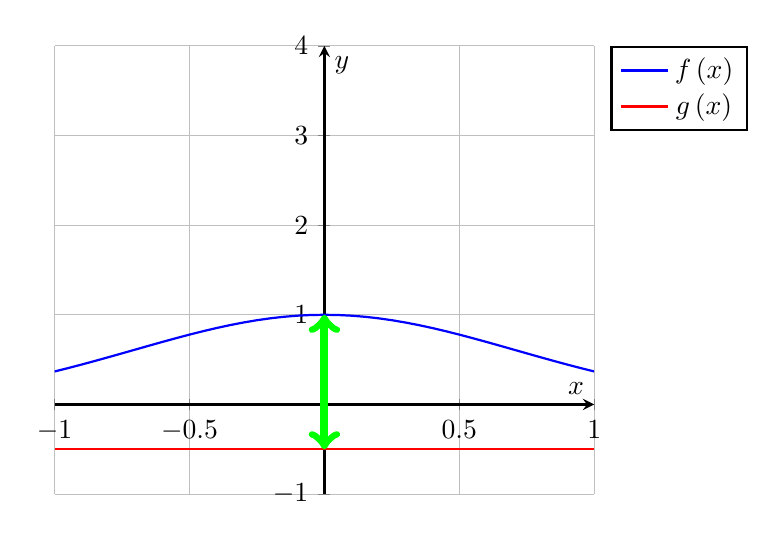
\begin{tikzpicture}[scale=1]
			\begin{axis}[
				xlabel={$x$},ylabel={$y$},
				axis lines=middle,
				samples=41,grid,thick,
				domain=-1:1,
				ymin=-1,ymax=4,
				legend pos=outer north east ]
				\addplot+[no marks] {e^-(abs(x*x))}; \addlegendentry{$f\left( x \right)$}
				\addplot+[no marks] {-0.5}; \addlegendentry{$g\left( x \right)$}
				\draw[<->,line width=1mm, color=green] (axis cs:0,-0.5) -- (axis cs:0,1);
			\end{axis}
		\end{tikzpicture}
\end{enumerate}
Si verificano le 4 proprietà di distanza:
\begin{enumerate}
	\item Se $\sup = \infty$ non va bene poiché l'insieme di arrivo è $\R$, applicando il Thm. di Weierstrass, una funzione continua definita su un intervallo $\realintervalclose{a}{b}$ ammette massimo e minimo e quindi anche il $\sup$ ....(le funzioni sono definite su un intervallo chiuso e limitato e sono continue)
	\item se e solo se hanno lo stesso dominio e per ogni punto di esso entrambe le funzioni hanno la stessa immagine
	\item $\dinfty{f}{g}=\ddinfty{f}{g}{\realintervalclose{a}{b}}=\ddinfty{g}{f}{\realintervalclose{a}{b}}=\dinfty{g}{f}$
	\item $\abs{h(x)-f(x)}\le\abs{h(x)-g(x)}+\abs{g(x)-f(x)} $, applicando il sup la disuguaglianza resta vera
\end{enumerate}
\observation 
Tutto questo è valido finché $\realintervalclose{a}{b}$ chiuso e limitato altrimenti non vale più Weierstrass \\
\\
UN CONTROESEMPIO\\
\\
\example
ferrovia
\example
Metrica Discreta
$X\ne \emptyset,\quad d(x,y)= \left\{\begin{matrix}0&&x=y\\0&&1\ne y\end{matrix}\right.$
	\begin{enumerate}
		\item $d(x,y)\ge 0$ per definizione
		\item $d(x,y)=0\iff x=y$, per definizione (ragiona sul sse) 
		\item $d(x,y)=d(y,x)$ ...per definizione (fai due casi x=y e l'altro)
		\item $d(x,y)\le d(y-z)+d(z-x)$ 
	\end{enumerate}
\example
$$X=\bbsetn{R}{2}$$
$$x=(x_1,x_2), y=(y_1,y_2)$$
$$d'(x,y)=\abs{x_1-y-1}+\abs{x_2-y-2}$$
...\\

\example
\example
$$X=\cntclass{0}(\realintervalclose{0}{1},\R)$$
$$d_2=\int_0^1\abs{g(x)-f(x)}d(x)$$
\example
$$X=\cntclass{0}(\realintervalclose{a}{b},\R), a,b\in\R, a<b$$
$$d_2=\sqrt{\int_a^b\left[g(x)-f(x)\right]^2d(x)}$$

\proposition
Sia $(X,d)$ s.m. e $A\subseteq X$ e $A\ne \emptyset$, sia $\begin{array}{rcl} d_{|A} : A\times A & \to & \mathbb{R} \\ (x,y) & \to & d(x,y) \end{array} \Rightarrow (A,d_{|A})$ è uno spazio metrico
\begin{proof}
	........
\end{proof}

\definition
Un insieme è finito se il numero dei suoi elementi è finito
\definition
Un insieme è infinito se non è finito
\definition
Sia $(X,d)$s.m., $A\subseteq X$, $A\ne \emptyset$ si definisce diametro di A: $$diam(A)=\sup\limits_{x,y\in A}d(x,y)$$
\definition
$A$ è limitato $\leftrightharpoons diam(A)$ è finito ($\in\R$)
\definition
$A$ è illimitato $\leftrightharpoons diam(A)$ è infinito ($=\infty$)
\example
...\\
...\\
...\\
..\\
....\\
\observation
Ogni insieme finito è limitato e ogni insieme illimitato è infinito. Non valgono i viceversa.
\example 
.....\\
....\\
.....\\
......\\
.....\\
....\\

\begin{definition}[Norma]
	\label{def:norma}
	Dato uno spazio vettoriale $V$ sul campo $\mathbb{K}$, si definisce \textbf{norma} una funzione $\norm{\cdot}:V\mapsto\R$ con le proprietà:
	\begin{enumerate}
		\item $\forall x\in V,\quad\norm{x}\ge0$
		\item $\forall x\in V,\quad\norm{x}=0\iff x=0$
		\item $\forall x,y\in V,\quad\norm{x+y}\le\norm{x}+\norm{y}$
		\item $\forall x\in V,\lambda\in\bbset{K},\quad\norm{\lambda x}=\abs{\lambda}\cdot\norm{x}$
	\end{enumerate}
	\begin{note}
		La funzione Norma associa dunque ad un vettore di qualsiasi dimensione uno scalare, fornendo (anche) una metrica per ordinare vettori tra loro.
	\end{note}
\end{definition}
\begin{definition}[Spazio Normato]
	Uno spazio normato è uno spazio vettoriale $V$ sul campo $\mathbb{K}$ \textbf{in cui è definita una norma}.
	\begin{note}
		Nel seguito verranno considerati esclusivamente spazi vettoriali su $\R$ o su $\mathbb{C}$, cioè $\mathbb{K} = \R$ o $\mathbb{K} = \mathbb{C}$
	\end{note}
\end{definition}
$X$ è uno spazio (vettoriale) normato sul campo $\bbset{K}$ se:
\begin{example}
$$X=\R\quad\norm{x}=\abs{x}$$
\end{example}
\begin{example}
	$$X=\bbsetn{R}{2}\quad\norm{\left[\begin{matrix}x\\y+\end{matrix}\right]}=\sqrt{x^2+y^2}$$
\end{example}
\begin{example}
	$$X=\bbsetn{R}{n}\quad x\equiv(x_1,\ldots,x_n)\quad \norm{x}=\sqrt{\sum\limits_{i=0}^n}x_i^2$$
\end{example}
\begin{example}
	$$X=\bbset{C}\quad\norm{x}=\abs{x}$$
\end{example}
\begin{example}
	$$X=\cntclass{0}(\realintervalclose{a}{b},\R)\quad\norm{f}\sup\limits_{x\in\realintervalclose{a}{b}}\abs{f}$$
\end{example}

\proposition
Sia $X$ uni spazio normato allora $(X,d)$ è uno spazio metrico con $\begin{array}{rcl} d : X\times X & \to & \mathbb{R} \\ (x_1,x_2) & \to & \norm(x_1-x_2) \end{array}$\\
Inoltre per la distanza così definita valgono le seguenti proprietà:
\begin{enumerate}
	\item INVARIANZA PER TRASLAZIONI
	$$\forall x_1,x_2,x_3\in X \quad d(x_1,x_2)=d(x_1+x_3,x_2+x_3)$$
	\item POSITIVAMENTE OMOGENEA
	$$ \forall x_1,x_2\in X, \lambda\in\R\quad d(\lambda x_1,\lambda x_2)=\abs{\lambda}d(x_1,x_2)$$
\end{enumerate}
\begin{proof}
	Per dimostrare che è uno spazio metrico si dimostra che valgono le proprietà di distanza
	\begin{enumerate}
		\item
		\item
		\item
		\item
	\end{enumerate}
\end{proof}

\definition
Sia $(X,d)$ spazio metrico e siano $x_0\in X$ e $r\in\bbset{r}$. Si dice sfera aperta di centro $x_0$ e raggio $r$ l'insieme:
$$B(x_0,r)=\left\{ x\in X : d(x,y)<r  \right\}$$
\observation
se $r=0\Rightarrow B(x_0,r)=\emptyset$\\
se $r>0\Rightarrow x_0\in B(x_0,r)$
\example
In $\R$ con $d_E$, $B(x_0,r)$ è un intervallo simmetrico centrato in $x_0$
\example
In $\bbsetn{R}{2}$ con $d_E$, $B(x_0,r)$ è una un cerchio con centro in $x_0$
\example
In $\bbsetn{R}{3}$ con $d_E$, $B(x_0,r)$ è una sfera con centro in $x_0$
\example

% TODO le definizioni prima di questa nel capitolo 1
\begin{definition}
	\label{def:aperto}
	Sia $(X,d)$ spazio metrico, sia $A\subseteq X$. Si definisce
	$$A\text{ è \textbf{aperto}}\bydef A=\emptyset\quad\text{oppure}\quad A=\circdot{A}$$
\end{definition}

\begin{definition}
	\label{def:chiuso}
	Sia $(X,d)$ spazio metrico, sia $A\subseteq X$. Si definisce
	$$A\text{ è \textbf{chiuso}}\bydef A=\emptyset\quad\text{oppure}\quad A=\bar{A}$$
\end{definition}

\definition
Siano $(X,d_1)$ e $(X,d_2)$ spazi metrici. $d_1$ e $d_2$ sono equivalenti $\leftrightharpoons \exists c,C\in\R, c_1>0, c_2>0$ t.c:
$$ \forall x,y \in X\quad cd_1(x,y)\le d_2(x,y)\le Cd_1(x,y) $$


\section{Successioni e Completezza}
\begin{definition}
	% TODO Definizione successione
\end{definition}
\begin{definition}
	% TODO Successione limitata
\end{definition}
\begin{definition}
	% TODO Successione convergente
\end{definition}
\begin{proposition}
	\label{prop:succ_conv_lim}
	Data la successione $x: \N \mapsto X$ di elementi dello spazio metrico $(X,d)$ e dato $x_\infty\in X$:
	$$\lim\limits_{n\rightarrow+\infty}x_n=x_\infty\iff\forall\varepsilon > 0\;\;\exists\nu\in\N:\quad\forall n>\nu\;\;d(x_n,x_\infty)<\varepsilon$$
	\begin{proof}
		% TODO dimostrazione
	\end{proof}
\end{proposition}
\subsection{Insiemi Compatti}
\begin{definition}[Insieme Compatto]
	\label{def:compatto}
	Sia $(X,d)$ uno spazio metrico e sia $A \subseteq X$. $A$ è compatto se e solo se ogni successione di elementi di $A$ ammette una sottosuccessione avente limite in $A$.
	\begin{note}
		Questa è la definizione di \textbf{Compattezza per Successioni}, in spazi più generali può essere necessario utilizzare una definizione più debole che, nel caso degli spazi metrici, coincide con la precedente.
	\end{note}
\end{definition}
\begin{exercise}
	\label{ex:unione_compatti}
	Sia $(X,d)$ uno spazio metrico. Siano $K_1$ e $K_2$ due sottoinsiemi compatti di $X$. Allora $K_1 \cup K_2$ è compatto
	\begin{solution}
		Posto $K = K_1 \cup K_2$, per definizione di \textbf{unione}, ogni elemento di $K$ è in $K_1$ o $K_2$.
		Visto che, per ipotesi, $K_1$ e $K_2$ sono compatti, sappiamo che ogni successione in uno dei due avrà una sottosuccessione convergente nello stesso insieme. A questo punto possiamo concludere che ogni successione in $K$ ammetterà una sottosuccessione convergente ad un elemento $x_\infty \in K_1$ oppure $x_\infty \in K_2 \implies x_\infty \in K$
	\end{solution}
\end{exercise}

\section{Limiti e Continuità}
\begin{definition}
	Siano $(X,d_x)$ e $(Y,d_y)$ spazi metrici, $A\subseteq{X}$,$x_0$ di accumulazione per $A$, $f:A\rightarrow{Y}$ una funzione e $l\in{Y}$ \\
	$\lim\limits_{x \rightarrow x_0} = l \rightleftharpoons \forall{\varepsilon},\exists\delta : \forall{x}\in A : d_x(x,x_0)<\delta e x\ne{x_0} : d_y(f(x),l)<\varepsilon$
\end{definition}

\begin{proposition}
	Siano $(X,d_x)$ e $(Y,d_y)$ spazi metrici, $A\subseteq{X}$,$x_0$ di accumulazione per $A$, $f:A\rightarrow{Y}$ una funzione e $l'\in{Y}$,$l''\in{Y}$
\end{proposition}

\begin{definition}[Funzione Continua]
	\label{def:funz_cont}
	Siano $(X,d_X)$ e $(Y,d_Y)$ spazi metrici e sia $f: A \mapsto Y$ con $A \subseteq X$ e sia $x_0 \in A$
	\begin{equation*}
		\begin{gathered}
			f \text{ è \textbf{continua} in } x_0 \iff\\
			\forall \varepsilon > 0\;\;\exists \delta > 0:\quad \forall x \in A \text{ con } d_X(x,x_0)<\delta \text{ vale } d_Y \bigl(f(x),f(x_0)\bigr) < \varepsilon
		\end{gathered}
	\end{equation*}

	\begin{center}
		$f$ è \textbf{continua} in $A\bydef$\\
		$f$ è continua \textbf{in ogni punto} di $A$
	\end{center}
	\begin{note}
		Non andrebbe detto semplicemente $f$ \textit{è continua} perché la continuità dipende in modo essenziale dall'insieme di punti su cui la funzione viene considerata. In assenza di ulteriori specificazioni, spesso si sottointende che l'insieme in esame è l'intero dominio della funzione.
	\end{note}
	\begin{note}
		Ha senso valutare la continuità di una funzione esclusivamente nell'insieme in cui è definita. Quindi una frase come:\\
		\textit{la funzione} $x \mapsto \frac{1}{x}$ \textit{è discontinua in} $0$,\\
		non è (a rigore) sensata. Andrebbe riformulata come:\\
		\textit{la funzione} $x \mapsto \frac{1}{x}$ \textit{non può essere estesa ad una funzione definita e continua anche in} $0$.
	\end{note}
	\begin{note}
		La continuità di una funzione dipende in modo esssenziale anche dalla distanza adottata, tuttavia è prassi sottointendere questa precisazione, soprattutto per funzioni $\R^n \mapsto \R^n$, se la distanza adottata è quella Euclidea.
	\end{note}
\end{definition}

\begin{theorem}[Teorema generale di Weierstrass]
	\label{teo:weier_generale}
	Siano $(X,d_X)$ e $(Y,d_Y)$ spazi metrici e sia $f:K \mapsto Y$ con $K \subseteq X$.
	$$\left.\begin{array}{ll}
		K \text{compatto} \\
		f \text{continua su } K
		\end{array} \quad\right\} \implies f(K) \text{compatto}$$
	\begin{proof}
		Siano le successioni
		\begin{itemize}
			\item $y: \N \mapsto Y$ tale che $y_n \in f(K) \;\forall n \in \N$, cioè $\forall n \in \N\;\exists x_n \in K: f(x_n) = y_n$
			\item $x: \N \mapsto X$ tale che $x_n \in K\;\forall n \in \N$
		\end{itemize}
		\begin{note}
			Abbiamo una successione che, attraverso la $f$ (non direttamente: le successioni non sono $X \mapsto Y$!), associa indirettamente valori in $K \subseteq X$ a valori in $f(K) \subseteq Y$
		\end{note}
		La successione $x$ ammette una sottosuccessione $x_{n_k}$ convergente ad un elemento $\overline{x} \in K$ dalla \fullref{def:compatto}, avendo $K$ compatto per ipotesi, ed essendo $x$ a valori in $K$.\\
		Data la continuità di $f$ in $K$, abbiamo $y_{n_k} = f(x_{n_k}) \in f(K)$, ma essendo $x_{n_k}$ convergente ad $\overline{x}$, anche $y_{n_k}$ converge, verificando così la definizione di spazio Compatto.
	\end{proof}
	\begin{proof} (Alternativa)\\
		La successione $x$ ammette una sottosuccessione $x_{n_k}$ convergente ad un elemento $\overline{x} \in K$, dunque da \fullref{prop:succ_conv_lim}:
		$$\lim\limits_{n\rightarrow+\infty}x_n=x_*\iff\forall\eta > 0\;\;\exists\nu\in\N:\quad\forall n>\nu\;\;d(x_n,x_*)<\eta$$
		Dalla \fullref{def:funz_cont} e sapendo che $f(x)$ è continua, sappiamo che:
		$$\forall\varepsilon > 0\;\;\exists\delta > 0:\quad\forall x \in K\;\;d_X (x,x_*)<\delta\;\;d_Y \bigl(f(x_n),f(x_*)\bigr)<\varepsilon$$
		Unisco ora le due definizioni:
		$$\forall \varepsilon > 0\;\;\exists \nu \in \N:\quad \forall n > \nu\;\;d_Y \bigl(f(x_n),f(x_*)\bigr)<\varepsilon$$
		Che equivale, per come è definita $y_n$, a
		$$\lim\limits_{n\rightarrow +\infty}y_n = y_*$$
		Cioè la definizione di successione convergente. Ho dunque individuato una sottosuccessione convergente per ogni successione in $f(K)$, verificando così la definizione di spazio Compatto.
	\end{proof}
\end{theorem}

\section{Il Teorema delle Contrazioni}
\begin{definition}[Contrazione]
	\label{def:contrazione}
	Sia $(X, d)$ uno spazio metrico. Si dice contrazione una funzione T: $X \mapsto X$ soddisfacente a:
	\begin{align}
		\label{equaz:def_contrazione}
		\exists K \in [0, 1[\;\text{tale che}\;\forall x',x''\in X\;\text{vale}\\
		d_X(T(x''), T(x')) \le K \cdot d_X(x'', x').
	\end{align}


	Una contrazione è quindi una funzione con insieme di partenza e di arrivo coincidenti e
	Lipschitziana con costante di Lipschitz strettamente minore di 1.
	E generalmente inutile considerare contrazioni definite tra spazi diversi. Data una funzione
	$T: X\rightarrow Y$ Lipschitziana, è sempre possibile riscalare la distanza in uno dei due spazi X o Y
	per ottenere una costante di Lipschitz minore di 1.
	\begin{note}
		D'ora in poi si utilizzerà la notazione $Tx$ per intendere $T(x)$
	\end{note}
\end{definition}

ESEMPI:\\
\begin{enumerate}
	\item $f: \R \rightarrow \R$ data da $f(x) = \frac{x}{2}$. $f$ è una contrazione.
	\item $f: [0,2] \rightarrow [0,2]$ data da $f(x) = 1+\frac{x}{2}. f$ è una contrazione
	\item $f: \R^2 \rightarrow \R^2$ data da $f(x,y)=\begin{bmatrix} \frac{1}{3}&&0\\0&&\frac{1}{5}\end{bmatrix}$ è una contrazione
\end{enumerate}

\proposition
Sia $(X, d)$ uno spazio metrico, siano $f,g:X\rightarrow X$ due contrazioni in $X \Rightarrow f\circ g$ è una contrazione
\begin{proof}
	Sappiamo che\\
	$$\forall x',x''\in X, d(fx'', fx')\le K_fd(x'', x').$$
	$$\forall x',x''\in X, d(gx'', gx')\le K_gd(x'', x').$$
	$f\circ g=f(g(x))$, quindi presi $x',x''\in X$ si ha che: $$d(fg(x''), fg(x'))\le K_fd(g(x''), g(x'))\le K_fK_gd(x'',x').$$
\end{proof}

\proposition
Sia $f \in C1(R^n;R^n)$. Se $\exists k \in [0, 1[$ tale che $\forall x \in \R^n$ vale $\norm{Df(x)}  < k$, allora $f$ è una contrazione.

\begin{theorem}[Teorema delle Contrazioni]
	\label{teo:contrazioni}
	Sia $(X, d)$ uno spazio metrico completo in cui è definita una contrazione
	$T: X \rightarrow X$. Allora esiste un unico punto fisso di $T$ in $X$.
	\begin{proof}
		Costruisco una successione di elementi di $X$ nel seguente modo:\\
		scelgo $x_0\in X$,\\
		$x_1 = Tx_0$\\
		$x_2 = Tx_1$\\\\
		...\\
		$x_n = Tx_{n-1}$\\
		La successione ${x_n: n \in N }$ così costruita è una successione di Cauchy. Infatti, presi $n, m \in N$ con $m > n$ si ha:
		$$d(x_{m},x_{n}) = d(Tx_{m-1},x_{n-1}) \le Kd(x_{m-1},x_{n-1})=$$
		$$=Kd(x_{m-1},x_{n-1}) = Kd(Tx_{m-2},x_{n-2}) \le K^2d(x_{m-2},x_{n-2})=$$
		$$=...=$$
		$$=...=K^nd(x_{m-n},x_{0})\le$$
		$$\le K^{n}\sum\limits_0^{m-n+1}(d(x_{m-n-i},x_{m-n-i-1}))=$$
		$$\le \sum\limits_0^{m-n+1}(d(Tx_{m-n-i-1},Tx_{m-n-i-2}))$$
		per ogni termine di questa sommatoria si può applicare lo stesso ragionamento
		$$\le K^{n}\sum\limits_0^{m-n+1}(K^{m-n-2}d(Tx_{0},x_{0}))=$$
		$$\le K^{n}d(Tx_{0},x_{0})\sum\limits_0^{m-n+1}K^{m-n-2}=K^n\frac{1-K^{m-n-1}}{1-K}d(Tx_{0},x_{0}) \le \frac{K^n}{1-K}d(Tx_{0},x_{0})$$
		Ho quindi trovato che $d(x_{m},x_{n})\le\frac{K^n}{1-K}d(Tx_{0},x_{0})$\\
		L’ultima espressione ottenuta può essere resa arbitrariamente piccola (in modulo) pur di
		prendere $n$, e quindi anche $m$, sufficientemente elevato. La completezza di $X$ implica quindi
		che esiste il limite $\lim\limits_{n\rightarrow +\infty}xn$. Sia $x^*$ questo limite. $x^*$ è un punto fisso per $T$. Infatti, grazie
		alla continuità di $T$:
		$$T(x^*)=T{\lim\limits_{n\rightarrow +\infty}xn}$$
	\end{proof}
\end{theorem}

\begin{definition}[Funzione Iterata]
	\label{def:iterata}
	Data $F:X\mapsto X$, si dice funzione iterata $n$ volte di $F$ la $F^n$ che corrisponde all'applicazione $n$ volte di $F$ su sè stessa. Formalmente:
	$$f^{n+1} = f \circ f^n \quad \forall n \in \N\setminus\brackets{0}$$
	Se $n = 0$, per definizione, $f^0 = \mathrm{Id}_X$ con $\mathrm{Id}_X$ funzione identità su $X$
\end{definition}

\begin{theorem}[Teorema dell'Iterata Contrazione]
	\label{teo:teo_iterata_contraz}
	Sia $(X,d_X)$ uno spazio metrico completo e sia $T:X\mapsto X : \exists n \in \N, T^n$ \textbf{iterata} è contrazione.\\
	Allora $T$ ammette un unico punto fisso in $X$
	\begin{note}
		La $n$ non è univocamente definita e non potrebbe esserlo. Se infatti $T^n$ è contrazione, allora anche $T^{2n},\, T^{3n},\, \cdots,\, T^{\alpha n}$ lo sono.
	\end{note}
	\begin{proof}
		Per il \fullref{teo:contrazioni} esiste un unico punto fisso $x_* \in X$ per $T^n$, quindi
		$$T^nx_* = x_*$$
		applicando $T$ ad entrambi i membri
		$$T(T^{n}x_*) = Tx_*$$
		e per la \fullref{def:iterata}
		$$T(T^{n}x_*) = T^n(Tx_*) = Tx_*$$
		Dunque $Tx_*$ è punto fisso della $T^n$. Avevamo però già trovato che $x_*$ era punto fisso della $T^n$ e, per il \fullref{teo:contrazioni}, può esistere un unico punto fisso. Ciò permette di concludere che $Tx_* = x_*$
	\end{proof}
\end{theorem}

\section{Funzioni a Valori in $\protect\mathbb{R}$}
%TODO This section is a placeholder